\begin{figure}[H]
    \centering
    \begin{subfigure}{0.4\textwidth}
        \centering
        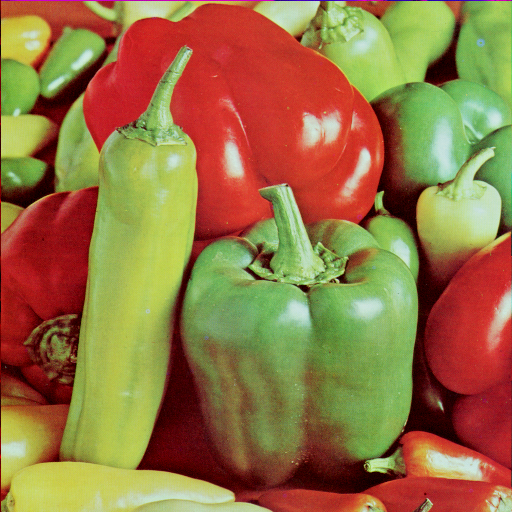
\includegraphics[width=0.85\textwidth]{pep_peq/imagem.png}
        \caption{Imagem com mensagem oculta.}
        \label{fig:pequeno:imagem}
    \end{subfigure}%
    \begin{subfigure}{0.4\textwidth}
        \centering
        \includegraphics[width=0.85\textwidth]{pep_peq/plano0.png}
        \caption{Plano 0.}
        \label{fig:pequeno:plano}
    \end{subfigure}\\[8pt]
    \begin{subfigure}{0.28\textwidth}
        \centering
        \includegraphics[width=0.85\textwidth]{pep_peq/pl0chb.png}
        \caption{Plano 0, canal azul.}
        \label{fig:pequeno:blue}
    \end{subfigure}%
    \begin{subfigure}{0.28\textwidth}
        \centering
        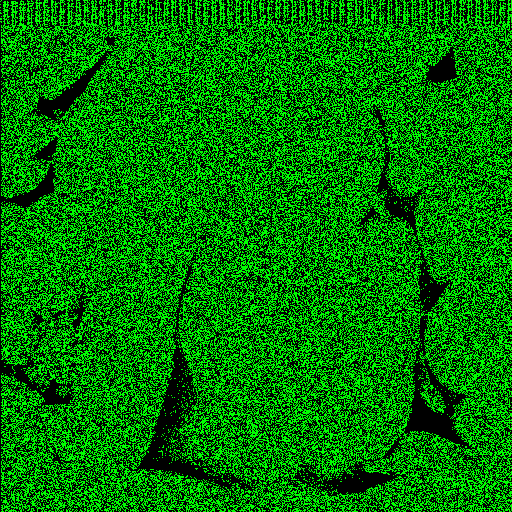
\includegraphics[width=0.85\textwidth]{pep_peq/pl0chg.png}
        \caption{Plano 0, canal verde.}
        \label{fig:pequeno:green}
    \end{subfigure}%
    \begin{subfigure}{0.28\textwidth}
        \centering
        \includegraphics[width=0.85\textwidth]{pep_peq/pl0chr.png}
        \caption{Plano 0, canal vermelho.}
        \label{fig:pequeno:red}
    \end{subfigure}%

    \caption{\texttt{peppers.png} com um texto de 4.5 KiB.}
    \label{fig:pequeno}
\end{figure}